\chapter{Použité součástky}
V této kapitole budou představeny a popsány součástky, se kterými budu v této ročníkové práci pracovat.

\section{ESP32-DevkitC}
%Co to je?
ESP32-DevKitC \cite{devkitc-datasheet} je malá programovatelná deska založená na čipu ESP32 od společnosti Espressiff \cite{espressif}. Vstupní a výstupní piny se nachází na obou stranách desky, což umožňuje uživateli připojit periferní zařízení jak pomocí propojovacích vodičů, tak připojením k~nepájivému poli. Na desce se také nachází mikro-USB port, který dovoluje  desku jednoduše napájet přímo z počítače, stejně jako nahrávat na desku soubory. \cite{devkitc}

\begin{figure}[htbp]
	\centering
	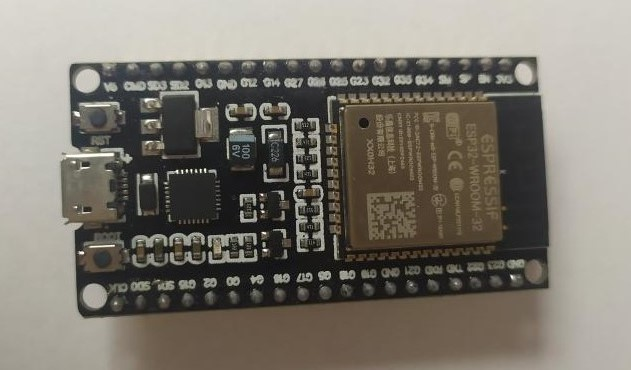
\includegraphics[width=0.5\textwidth]{img/ESPDevKit3.jpg}
	\caption{ESP32-DevKitC}
	%	\label{fig:install-sdk-3}
\end{figure}

%Co se s tím dá dělat
Deska je kompatibilní s Arduinem \cite{arduino} a často se v kombinaci zrovna s~tímto typem desek používá. Díky zabudovanému Wifi modulu, který nese čip ESP32,\cite{ESP32} je možné se na~součástku napojit a používat jakékoliv zařízení pracující s Wifi (například chytrý mobilní telefon), aby se k součástce napojilo a fungovalo jako dálkový ovladač. V praxi jsem se nejčastěji setkala s použitím mobilního telefonu jako dálkového ovladače právě v případě výše zmíněného programování LED světel a řízení drobného robota. S ESP32-DevkitC se dá dělat ale prakticky cokoliv: například se dá použít jako procesor pro po domácku vyrobený alarm, amatérský anemograf na zaznamenávání počasí nebo právě pro  vyrobení malého pojízdného robota na dálkové ovládání. 
%todo Otázka --> udělat čip ESP32 proklikávací, nebo ho nechat v literatuře tak, jak je?

 \href{https://www.espressif.com/sites/default/files/documentation/esp32_datasheet_en.pdf}{ESP32}

%Proč jsem si vybrala zrovna tuto součástku.
Já jsem se rozhodla použít ESP32-DevKitC kvůli jeho dostupnosti, všestrannému využití a taky (možná hlavně) proto, že v mém okolí mělo spoustu lidí s~touhle technologií zkušenosti a mohli mi v případě nějakého problému jednoduše pomoci. 
Plánovala jsem, že Wifi modul na této desce jednoduše využiji pro dálkové ovládání ESP32-DevKitC z mobilního telefonu. Rozměry desky ESP32-DevkitC (přibližně 55 mm na 30 mm) byly také vyhovující pro pozdější teoretické vybudování napájecí \emph{základny}, která měla napájet a řídit LED schované v~průhledné plastové květině.
%todo --> Otázka --> může být označení základna kurzívou?


%todo Neopixel distributor
\section{NeoPixel modul s 8 RGB LED WS2812}
%Co to je? Co se s tím dá dělat
Jedná se o pevný pásek s inteligentními LED za sebou. Často se využívá jako výstupní model pro Arduino a obsahuje 8 RGB LED typu WS2812,\cite {WS2812} které lze najít i pod označením NeoPixel\cite{Neopixel}. Výhoda tohoto LED pásku je, že se dá řídit pomocí jednoho datového pinu a~dvou napájecích pinů, což umožňuje kontrolér ve WS diodách. Tento modul se sice nehodí našemu původnímu záměru, který vyžaduje aby LED byly na pásku ohebném, ale jako modul pro testování stačí.

%todo Otázka --> V jakém čase mám psát text? Je to vyhovující tak, jak to je?

\begin{figure}[htbp]
	\centering
	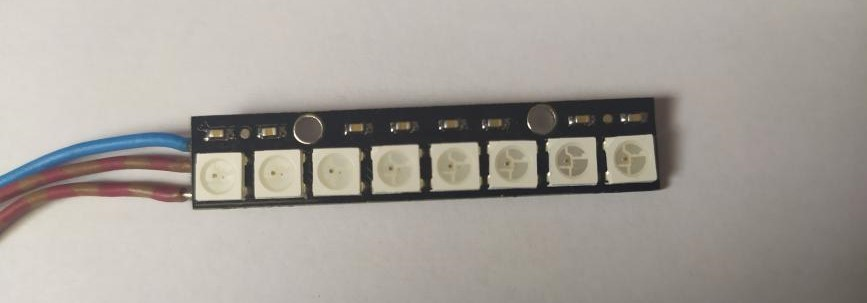
\includegraphics[width=0.5\textwidth]{img/NeoPixel2.jpg}
	\caption{NeoPixel modul}
	%	\label{fig:install-sdk-3}
\end{figure}

%Proč jsem si vybrala zrovna tuto součástku.
Tuto součástku jsem se rozhodla použít ze dvou důvodů. Ten první byl, že jsem ještě nevěděla jistě, jaký ohebný LED pásek bych chtěla použít. Druhý důvod byl stejný, jako v~případě ESP32. A to, že kdyby nastaly při práci s tímto modulem nějaké problémy, tak jsem znala spoustu lidí, kteří by mi s případnými problémy dokázali pomoci.

\newpage

\section{Pásek WS2812 ohebný}
Po nějaké době práce s předchozím LED páskem jsem si nakonec rozhodla vybrat skoro totožný pásek až na určitou maličkost, a to, aby byl jednoduše ohebný a tvarovatelný. Pracuje a programuje se s ním stejně, jako s předchozím páskem, avšak, jelikož to více vyhovovalo mému záměru, jsem tentokrát použila pásek se čtyřmi RGB LED.\cite{Ohebny}
%todo --> Otázka --> Můžu si dovolit odkaz na amazon? Nemůžu najít oficiálního distributora

\begin{figure}[htbp]
	\centering
	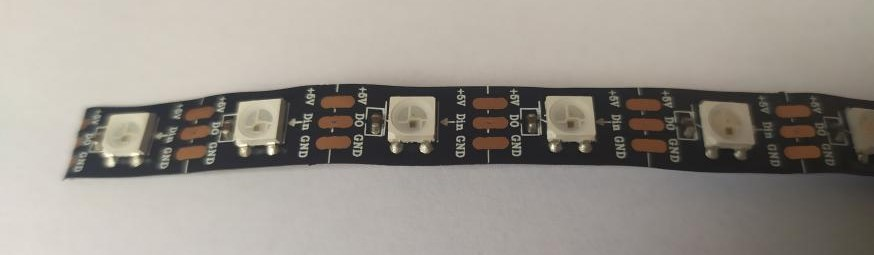
\includegraphics[width=0.5\textwidth]{img/OhebnyLedPasek2.jpg}
%<<<<<<< Updated upstream
	\caption{Pásek WS2812}
%=======
%	\caption{Pásek ws2812}
%>>>>>>> Stashed changes
	%	\label{fig:install-sdk-3}
\end{figure}


\section{Pájení}

Proto, abych s těmito součástkami mohla dál pracovat, jsem potřebovala napojit pevný LED NeoPixel pásek na ESP32-DevKitC. Což jsem udělala tak, že jsem k Neopixel pásku připájela dráty na kontakty: napájení, uzemění a vstupní pin. Na tyto dráty jsem z~druhé strany přidělala pinhead a napojila jsem jej z druhé strany na ESP32-DevKitC. Jako vstupní pin jsem zvolila pin č. 21.  

\begin{figure}[htbp]
	\centering
	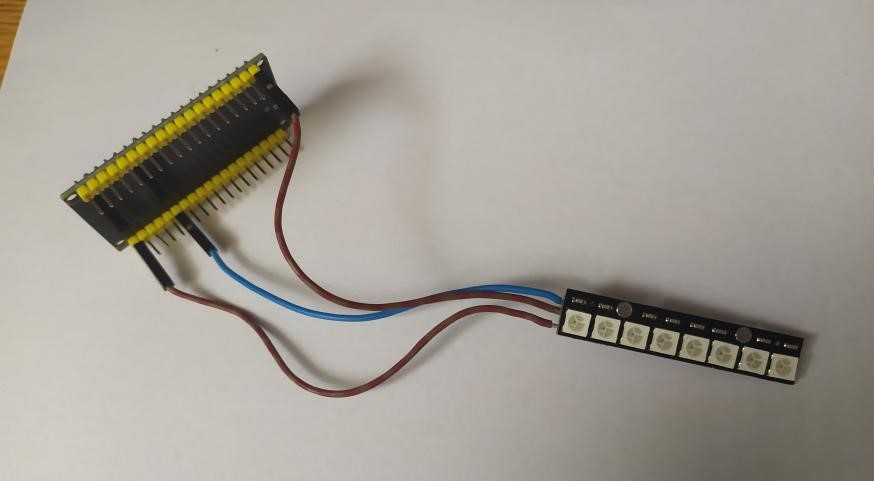
\includegraphics[width=0.5\textwidth]{img/Zapájené2.jpg}
	\caption{Zapájený NeoPixel, připojený k ESP32-DevkitC}
	%	\label{fig:install-sdk-3}
\end{figure}


Zde jsou zapájené součástky. Po tomto kroku jsem se mohla pustit do programování.

%Ostatní poznámky:
%Deska má tři druhy napájení, ale já budu využívat pouze napájení zkrz mikro-USB protože je to pro mě nejjednodušší. Stejně tak do toho budu posílat nahrané soubory z počítače
%Je potřeba vymyslet systém napájení
%Jak to funguje? Jaké je rozložení dané desky? 
